\documentclass{standalone}
\usepackage{tikz}
\usepackage{amsmath}
\usetikzlibrary{decorations.markings}

\begin{document}
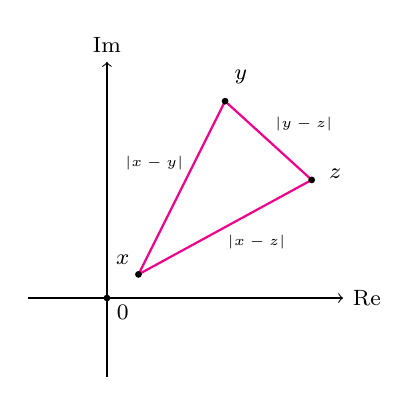
\begin{tikzpicture}
  \draw[->] (-1,0) -- (3,0) node[right] {\footnotesize$\operatorname{Re}$};
  \draw[->] (0,-1) -- (0,3) node[above] {\footnotesize$\operatorname{Im}$};
  


\draw[magenta, thick] (1.5,2.5) -- (2.6,1.5);

\draw[magenta, thick] (0.4,0.3) -- (1.5,2.5);

\draw[magenta, thick] (0.4,0.3) -- (2.6,1.5);


   \filldraw (1.5,2.5) circle (1pt);
    \node[anchor=south] at (1.7,2.6) {\footnotesize$y$};


   \filldraw (0.4,0.3) circle (1pt);
    \node[anchor=south] at (0.2,0.3) {\footnotesize$x$}; 
 
   \filldraw (2.6,1.5) circle (1pt);
    \node[anchor=south] at (2.9,1.4) {\footnotesize$z$}; 
  
  
  \filldraw (0,0) circle (1pt);
  \node[anchor=south] at (0.2,-0.4) {\footnotesize$0$};
  
  
 \node[anchor=south] at (2.5,2.0) {\tiny$|y - z|$}; 
  \node[anchor=south] at (1.9,0.5) {\tiny$|x - z|$}; 
   \node[anchor=south] at (0.6,1.5) {\tiny$|x - y|$}; 
  
\end{tikzpicture}
\end{document}